\documentclass[uplatex,dvipdfmx,11pt,notheorems,aspectratio = 169]{beamer}
\usepackage{comment}
\usepackage{color}
\usepackage{nccmath}
\usepackage{hyperref}

%%%% 和文用 %%%%%
\usepackage{bxdpx-beamer}
\usepackage{pxjahyper}
%\usepackage{minijs}%和文用 pLaTeX用

\renewcommand{\kanjifamilydefault}{\gtdefault}%和文用
% \newcommand{\g}[1]{\mathtt{#1}}
\newcommand{\tup}[1]{\left\langle{#1}\right\rangle}

%%%% スライドの見た目 %%%%%
\usetheme{Frankfurt}
\usecolortheme[accent=cyan]{solarized}
\usefonttheme{professionalfonts}
\setbeamertemplate{frametitle}[default][left]
\setbeamertemplate{navigation symbols}{}
\setbeamercovered{transparent}%好みに応じてどうぞ)
\setbeamertemplate{footline}[page number]
\setbeamerfont{footline}{size=\normalsize,series=\bfseries}
%%%%

%%%% 定義環境 %%%%%
\usepackage{amsmath,amssymb}
\usepackage{amsthm}
\usepackage{mathtools}
\usepackage{bussproofs}
\usepackage{physics}
\theoremstyle{definition}
\newtheorem{theorem}{定理}
\newtheorem{definition}{定義}
\newtheorem{proposition}{命題}
\newtheorem{lemma}{補題}
\newtheorem{corollary}{系}
\newtheorem{conjecture}{予想}
\newtheorem*{remark}{Remark}
\renewcommand{\proofname}{証明}
%%%%%%%%%

%%%%% フォント基本設定 %%%%%
\usepackage[T1]{fontenc}%8bit フォント
\usepackage{textcomp}%欧文フォントの追加
\usepackage[utf8]{inputenc}%文字コードをUTF-8
\usepackage{otf}%otfパッケージ
% \usepackage{newpxmath}%数式・英文ローマン体を newpxmath にする
\usepackage{bm}%数式太字
%%%%%%%%%%

% \makeatletter
% \def\BOXSYMBOL{\RIfM@\bgroup\else$\bgroup\aftergroup$\fi
%   \vcenter{\hrule\hbox{\vrule height.85em\kern.6em\vrule}\hrule}\egroup}
% \makeatother
% \newcommand{\BOX}{%
%   \ifmmode\else\leavevmode\unskip\penalty9999\hbox{}\nobreak\hfill\fi
%   \quad\hbox{\BOXSYMBOL}}
% \renewcommand\qed{\BOX}

% 図の絶対座標指定
\usepackage[absolute,overlay]{textpos}
% \usepackage[colorgrid,gridunit=pt,texcoord]{eso-pic}
% 図の入れ方
% \begin{figure}[H] % h...hereの意
%   \centering
%   \includegraphics[width=15cm]{kairo.png}
%   \caption{キャプション名\label{ラベル名}}
% \end{figure}
% 図の入れ方(絶対座標指定)
% \begin{textblock*}{0.7\linewidth}(50pt,50pt)
%   \centering
%   \includegraphics[width=\linewidth]{2-7.jpg}
% \end{textblock*}

% 回り込む図
% \begin{wrapfigure}[13]{r}{5cm}
%   \centering
%   \includegraphics[width=5cm]{img/schematics.png}
%   \vspace*{-\intextsep}
%   \caption{システムの模式図\label{schematics}}
% \end{wrapfigure}

% 表の入れ方
% \begin{table}[H]
%   \centering
%   \caption{キャプション名\label{ラベル名}}
%   \begin{tabular}{c|c|c|c} \hline \hline
%     抵抗名 &$\zeta$ &$\psi$ & $g :\ \mathrm{dB}$ \\\hline
%     R1&$0.0500$ &$ 0.997 $ & $20.0$\\\hline
%     R3 & $0.500$ &$0.707$ & $2.32$ \\\hline
%   \end{tabular}
% \end{table}

% pdf 挿入の仕方
% \includepdf[pages=-]{pdfs/reviews.pdf}
% \includepdf[pages=3]{pdfs/FrontCovers.pdf}
% \includepdf[pages=2-]{pdfs/report1.pdf}

% caption に番号追加
\setbeamertemplate{caption}[numbered]

\title[略タイトル]{ReDoS脆弱な正規表現の修正}%[略タイトル]{タイトル}
\author[富家]{富家 功一朗}%[略名前]{名前}
\institute[JPN]{早稲田大学基幹理工学部情報理工学科}%[略所属]{所属}
\date{\today}%日付


\begin{document}

\begin{frame}[plain]\frametitle{}
\titlepage %表紙
\end{frame}

\begin{frame}\frametitle{目次}
\tableofcontents %目次
\end{frame}


\section{ReDoS脆弱性}
\begin{frame}
  \begin{itemize}
    \item ReDoSとは何か?
    \item regular expression denial of serviceの略.
    \item 正規表現のパターンマッチの脆弱性を利用したDoS攻撃(ウェブサイトやサーバーに負荷をかけ,その可用性を侵害する行為)のこと.
  \end{itemize}
\end{frame}

\begin{frame}
  ReDoS脆弱性を孕んだ正規表現を用いた結果,以下のような事例が発生している.
  \begin{itemize}
    \item 2016年,Stack Overflowのサーバーが,空白を2万個含む投稿によりダウンした\cite{stackoverflow}.
    \item 2019年,Cloudflareが提供するCDNが,ファイヤーウォールに追加した脆弱性な正規表現によりダウンした\cite{cloudflare}.
  \end{itemize}
\end{frame}

\begin{frame}
  では,正規表現のパターンマッチの脆弱性とは一体何なのだろうか?
\end{frame}

\begin{frame}
  \begin{itemize}
    \item そもそも正規表現のパターンマッチ処理はその正規表現に対応するNFAをバックトラック探索することにより行われている.
  \begin{figure}[H] % h...hereの意
    \centering
    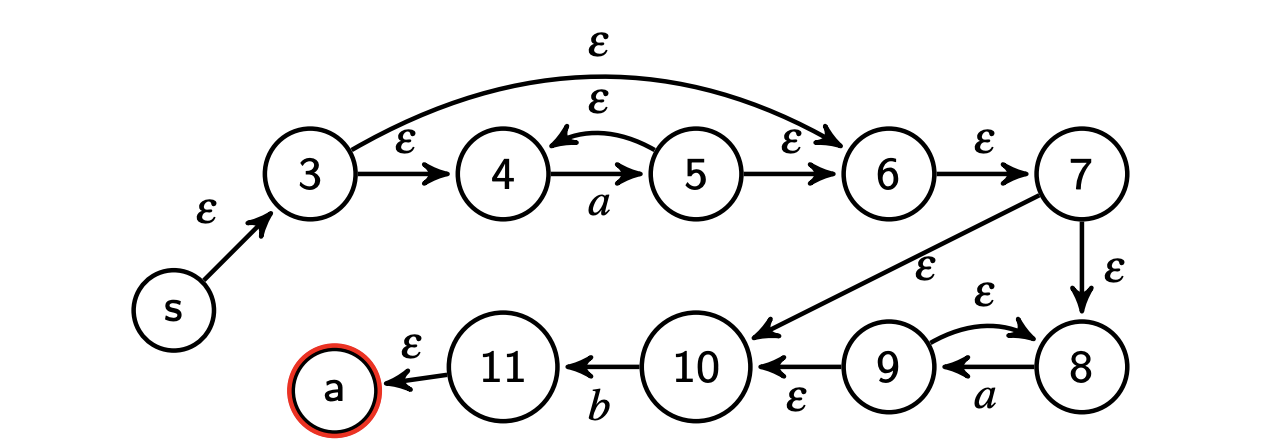
\includegraphics[width=0.75\linewidth]{a*a*b.png}
  \end{figure}
    \item 上記の図は正規表現$a^*a^*b$に対応するNFAである(\cite{javascript}より引用).
    \item $aaa$という文字列は$a^*a^*b$に受理されないが,このときどのようなパターンマッチ処理が発生するのかを見る.
  \end{itemize}
\end{frame}

\begin{frame}
  \begin{itemize}
    \item まず,初期状態$s$から遷移できるところまで進む.今回の例では初期状態$s$から$a$という文字を2つ消費した後の状態10までは遷移できる.以下はそのようなパス.
    \begin{equation}
      (s,\varepsilon,3),(3,\varepsilon,4),(4,a,5),(5,\varepsilon,6),(6,\varepsilon,7),(7,\varepsilon,8),(8,a,9),(9,\varepsilon,10)\label{path1}
    \end{equation}
    \item しかし,状態10から先へは文字$b$がなければ進めない.
    \item このような状況に陥った際,1手前に戻る,すなわち\textcolor{red}{バックトラック}が行われる.
    \item 具体的に言えば,(\ref{path1})の探索パスで言えば状態10から進めないことが分かったので状態9に戻ってやり直すということである.状態9に戻って,残りの文字$a$を読み取った上で状態$a$にたどりつけるようなパスを探すが存在しないので,またバックトラックする.
  \end{itemize}
\end{frame}

\begin{frame}
  このように文字列のパターンマッチングではバックトラックを繰り返し行うことが多々ある.そして,バックトラックの回数が文字列のパターンマッチングの実行時間に大きな影響を与える.
\end{frame}


\section{脆弱な正規表現の修正}
\begin{frame}
  ここからは脆弱な正規表現を修正する方法について見ていく.まず,本研究で提案する手法ではREMEDY,RegEqという2つのプログラムを利用するのでそれらの説明を行う.
\end{frame}



\subsection{ベースとなるプログラムの説明}
\begin{frame}{ベースとなるプログラムの説明}
まず,RegEq\cite{regeq}について説明を行う.\vspace{0.2in}

2つの正規言語を入力としたとき,それらが意味的に等価であるかを判定する.意味的に等価というのは,受理する文字列の集合が等しいということ.等価でなかった場合,片方の正規言語には受理されるが,もう片方の言語には受理されない文字列が反例として返される.\vspace{0.2in}

RegEqでは2つの正規言語をDFAに変換し,差を取り,それが空であるかどうかを判定することにより,等価性判定が行われている.
\end{frame}

\begin{frame}{ベースとなるプログラムの説明}
次に,REMEDY\cite{remedy}について説明を行う.\vspace{0.2in}

REMEDYは正規表現とpositive example(正例)とnegative example(負例)を入力として与えると,以下の条件を満たすような正規表現を出力として返す.
\begin{enumerate}
  \item 入力として与えられたpositive example,negative exampleが正しく分類されている(positive exampleは受理され,negative exampleは受理されない)
  \item real-world strong 1-unambuiguity(RWS1U)
  \item 入力として与えられた正規表現に構文的に近い
\end{enumerate}
\vspace{0.2in}
\begin{itemize}
  \item RWS1Uを満たせば正規表現が非脆弱であることが保証される.
  \item あくまで修正後の正規表現が与えられた例を判別する能力を持つだけで,修正前の正規表現と後の正規表現が\textcolor{red}{意味的に等しいとは限らない}.
\end{itemize}
\end{frame}



\subsection{提案手法}
\begin{frame}{提案手法}
  上記の2つのプログラムを用いて以下のようなアルゴリズムで正規表現を意味的な等しさを保ったまま非脆弱化する.
  \begin{enumerate}
    \item (ReDoS脆弱だと疑われる)正規表現をREMEDYへの入力とする.はじめはpositive example,negative exampleともに入力として渡さない(つまりpositive exampleの集合,negative example集合がともに空である).
    \item REMEDYから出力された正規表現と元の正規表現をRegEqへの入力とし,
    \begin{itemize}
      \item 等価であるなら修正後の正規表現を返してこのアルゴリズムは終了.
      \item 等価でないなら元の正規表現に受理され修正後の正規表現に受理されない文字列を正例に追加し,元の正規表現に受理されず修正後の正規表現に受理される文字列を負例に追加し,それらを修正後の正規表現とともにREMEDYに渡す.
    \end{itemize}
    \item 2.を繰り返す.
  \end{enumerate}
  なお,このアルゴリズムは停止しない場合がある.なぜなら,ある正規表現に対してそれを表しかつS1Uを満たすような正規表現がない正規言語が存在するからである.
\end{frame}

\begin{frame}
  上記のアルゴリズムを直感的に表した図を以下に示す.
  \begin{figure}[H] % h...hereの意
    \centering
    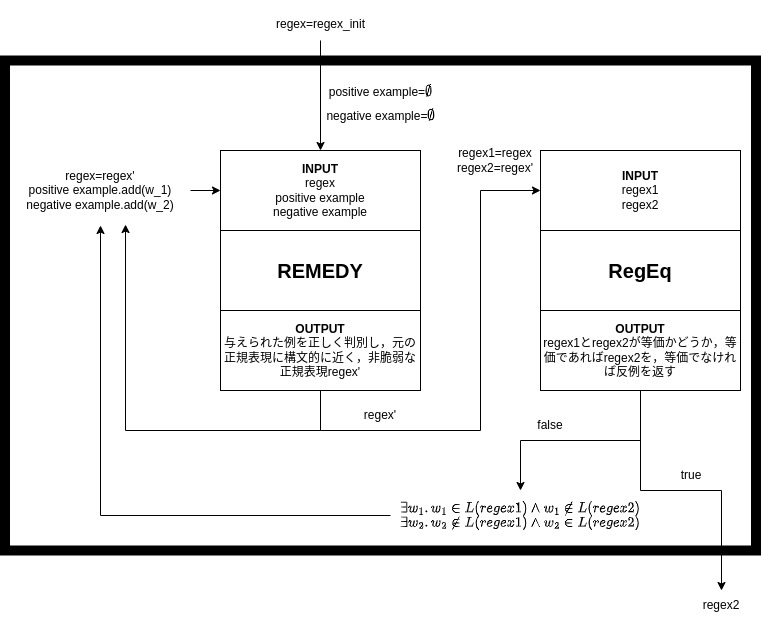
\includegraphics[width=0.65\linewidth]{seminar.jpg}
    % \caption{脆弱なNFAのパターン\label{ラベル名}}
  \end{figure}
\end{frame}

\begin{frame}{実験}
  脆弱な正規表現$c(ab)^*a(ba)^*$と$.^*a^*\mathrm{=}$に本アルゴリズムを適用してみる.その結果は以下の通り.
  \begin{table}[H]
    \centering
    \caption{脆弱な正規表現$c(ab)^*a(ba)^*$の修正結果\label{vul_res1}}
    \begin{tabular}{c|c|c} \hline \hline
        修正前の正規表現 & 修正後の正規表現  & 修正にかかった時間[s]\\\hline
        $c(ab)^*a(ba)^*$  & $ca(ba)^*$ &$0.533$ \\\hline
    \end{tabular}
  \end{table}

  \begin{table}[H]
    \centering
    \caption{脆弱な正規表現$.^*a^*\mathrm{=}$の修正結果\label{vul_res2}}
    \begin{tabular}{c|c|c} \hline \hline
        修正前の正規表現 & 修正後の正規表現  & 修正にかかった時間[s]\\\hline
        $.^*a^*\mathrm{=}$  & $[\mathchar`^\mathrm{=}]^*\mathrm{=}([\mathchar`^\mathrm{=}]^*\mathrm{=})^*$ &$55.000$ \\\hline
    \end{tabular}
  \end{table}
\end{frame}

\begin{frame}
  \begin{itemize}
    \item 今回は比較的短時間で終わる例のみ取り上げた.1時間かけても終わらない例もあった.
    \item REMEDYは文字列例を元に正規表現を構成するPBE(programming by example)という手法を取っているため,適切な例を持ってこれるか否かが本プログラムの実行速度に影響を及ぼす.
    \item だが,どのような例を持ってくれば早く目的の正規表現を得られるのかはよく分かっていないので今後の課題としたい.
  \end{itemize}
\end{frame}




\begin{frame}[allowframebreaks]{Reference}
  \scriptsize
  \beamertemplatetextbibitems
  \bibliographystyle{junsrt}
  % \bibliographystyle{jplain}
  \bibliography{main}
\end{frame}



\end{document}